\documentclass{article}
\usepackage{graphicx}
\usepackage{amsmath}
\usepackage{tikz}
\title{ODE and Diffusion Models of Tumor Growth}
\author{Daniel Henricks}


\begin{document}

\maketitle

\section{Introduction}

Researchers have been studying cancer and the patterns behind tumor growth for thousands of years. Hippocrates
was accredited with possibly being the first to describe a tumor, and tumors were mainly described by their color
and their response to touch. However, ancient physicians did not separate benign and malignant tumors, but they
acknowledged the tumor's ability to infect nearby tissue. The application of mathematical models to tumor growth
did not start to gain traction until much later, however. In the early 20th century, one of the most famous uses of
the diffusion model was first developed: Hill released a paper discussing how the movement of lactic acid
and oyxgen throughout the body could be shaped into a diffusion problem (Hill, 1928). This paper eventually led to
Greenspan's paper which modeled the growth of tumors using diffusion, applying many of the mathematical tools employed
by Hill some years before (Greenspan, 1972). This paper will present a brief overview of the mathematics used in these
papers and will recreate some of the graphics produced as well.

\section{Hill's Paper}

Hill's paper, titled `Diffusion of Oxygen and Lactic Acid through Tissues', set the scene for most of the diffusion models
developed in the late 20th century to present. In the introduction of this paper, Hill states that the
`diffusion of dissolved substances through cells and tissues is a determining factor in many vital processes'.
The diffusion constant, $k$, is introduced, along with its usages. It is representative of the number of unit quantities
of a substance that diffuse throughout an area of 1 $cm^2$ in a minute. The diffusion constant is usually a small value
when related to systems that are outside of the body; for example, the diffusion constant would be very small when studying
the diffusion of a gas within a large room. However, when studying systems within the body, the diffusion constant can be quite large.
Hill gives the following example when explaining this:

\begin{tabular}{|c|c|c|}
    \hline
    Object             & Diameter            & Time to 90\% Saturation \\
    \hline
    Cylinder           & 1 cm                & 185 minutes             \\
    Actual Nerve       & 0.7 mm              & 54 seconds              \\
    Single Nerve Fiber & 7 $\mu$ (0.0007 cm) & 0.0054 seconds          \\
    \hline
\end{tabular}
\vspace*{1cm}

As seen by this example, many processes of diffusion throughout the body are extremely rapid. However, at the time of Hill's
paper, another problem was evident: not many problems in diffusion could be completely solved using mathematical methods.
Even when evaluating these equations, the existence of a unique solution was only guaranteed with certain inital conditions.
The steady state also needed to have specific parameters in order for the result to be of any interest.
\subsection{Diffusion of Oxygen Within a Steady State}

The first problem that Hill dealt with was the case where oxygen was being diffused from a gaseous or liquid phase.
It was assumed that the oxygen was being used up by metabolic processes at some rate $a$ and that the concentration
of oxygen, $y_0$, is maintained constant at $x = 0$.

\vspace*{0.5cm}

Let $x$ be the distance from the constant source of oxygen to any point within the tissue. Given the assumptions above,
the rate of diffusion across any unit area will be $ J = -k \* \frac{dy}{dx}$,\, where $J$ is the rate of diffusion, $k$ is the diffusion rate and the (-)
represents that the diffusion is occuring in the opposite direction from the source. This is more commonly known as Fick's
first law of diffusion. To find the measure of this rate of accumulation, Fick's second law can be applied:
\begin{equation}
    \frac{dJ}{dx} = k \* \frac{d^2y}{dx^2}
\end{equation}

Hill then combined these equations along with $a$, the rate of usage by the metabolic process, to come up with the first diffusion equation for
this model:

\begin{equation}
    \frac{dy}{dt} + a = k \* \frac{d^2y}{dx^2}
\end{equation}

This equation states that the rate of change of the concentration of oxygen plus the rate of usage of the oxygen is equal to the diffusion equation.
Note that from the assumptions above, the concentration is held constant, so the equation can be further simplified to:

\begin{equation}
    a = k \frac{d^2y}{dx^2}
    \label{eq:oxygen}
\end{equation}

The solution of the equation is

\begin{equation}
    y = \frac{ax^2}{2k} + bx + y_0
\end{equation}

where $b$ is a constant.
This can be verified by taking the derivative of this equation twice:

$ \frac{dy}{dx} = \frac{a}{k}x + b$,

\vspace*{0.25cm}

$ \frac{d^2y}{dx^2} = \frac{a}{k}$
\vspace*{0.25cm}

To find the value of b that satisfies these equations, we assume that there must be some point
very far away from the source where the concentration is zero and the diffusion of oxygen is not occuring,
so $\frac{dy}{dx}$ is also equal to zero.


We define $x'$ as the minimum distance where the concentration is equal to zero and then set these two equations equal to zero and solve:

\vspace*{0.25cm}
$ 0 = \frac{a{x'}^2}{2k} + bx' + y_0 $
\vspace*{0.25cm}

$ 0 = \frac{ax'}{k} + b \Leftrightarrow b = -\frac{ax'}{k}$
\vspace*{0.5cm}

Substituting back into the first equation:
\vspace*{0.5cm}

$ 0 = \frac{a{x'}^2}{2k} - \frac{a{x'}^2}{k} + y_0 \Leftrightarrow y_0 = \frac{a{x'}^2}{2k}$

So
\begin{equation}
    x' = \sqrt{\frac{2ky_0}{a}}
\end{equation}
(the maximum permeation distance of the oxygen from the source)

and

\begin{equation}
    b = \sqrt{\frac{-2ay_0}{k}}
\end{equation}

We can now solve to find how much oxygen has been absorbed by the tissue: $ \int_{0}^{x'} y dx $, where y is found in
equation (3).

We get the integral:

\begin{equation}
    Y = \int_{0}^{\sqrt{\frac{2ky_0}{a}}} \frac{ax^2}{2k} + bx + y_0 dx
\end{equation}

To solve (7), we integrate and then simplify:

\vspace*{0.25cm}

$Y = \frac{ax^3}{6k} - \frac{x^2}{2}\sqrt{\frac{2ay_0}{k}} + y_0x \Bigg|_0^{\sqrt{\frac{2ky_0}{a}}}$
\vspace*{0.25cm}

$ = \sqrt{2ky_0} \frac{y_0}{3\sqrt{a}} - \frac{ky_0\sqrt{\frac{2ay_0}{k}}}{a} + y_0\sqrt{\frac{2ky_0}{a}}$
\vspace*{0.25cm}

\begin{equation}
    = y_0 \frac{x'}{3}
\end{equation}

This result (which Hill also derived) shows that the maximum absorption of oxygen in a tissue that is $x'$ thick
is one-third the full amount of oxygen that is diffused.

\subsection{Diffusion of Lactic Acid Within a Steady State}


This case is the exact opposite of the case studied above. As the tissue uses up the oxygen, lactic acid is built up
at a rate of $-\alpha$, the opposite sign as seen in equation (3) above. So our equation then becomes

\begin{equation}
    -\alpha = k' \frac{d^2y'}{dx^2}
    \label{eq:lactic_acid}
\end{equation}

where $k'$ is the new diffusion constant of lactic acid and $y'$ is the concentration of lactic acid at any point $x$.
Using the same processes as above, we can find a solution to this equation:

\begin{equation}
    y' = \frac{-\alpha x^2}{2k'} - \beta x + y_0'
\end{equation}

and can find that the total amount of lactic acid dissolved is

\begin{equation}
    Y = \frac{y_0' \beta}{3}
\end{equation}

These equations all assume that there exists some point in the tissue where the concentration of lactic acid or oxygen
is equal to zero. If this is not the case, Hill showed in his paper that the amount of oxygen dissolved would be

\begin{equation}
    y_0b - \frac{ab^3}{3k}
\end{equation}

and the total amount of lactic acid dissolved would be

\begin{equation}
    y_0'b + \frac{\alpha b^3}{3k'}
\end{equation}

\subsection{Combining Oxygen and Lactic Acid Diffusion}

Hill then combined both equations to come to a conclusion on how lactic acid and oxygen would interact in a muscle.

The conclusions made from this section of the paper were essential for future models of diffusion. First, it was
assumed that the thickness $b > x'$ so none of the oxygen was able to penetrate through the entire system. From above,
the concentrations of oxygen and lactic acid are $y$ and $y'$ respectively. The plane sheet of tissue will have oxygen
at a partial pressure of $y_0$ from the left and an impenetrable wall on the right. Also let $a$ be the rate of usage
(in cubic centimeters of tissue) of oxygen by the tissue.
Then the following graphic describes the system:

\begin{figure}[h!]
    \centering
    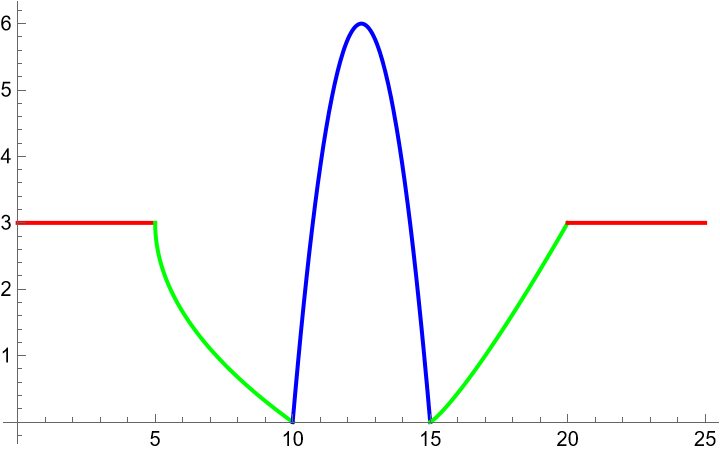
\includegraphics[width=0.9\textwidth]{graphics/image.png}
    \caption{From 0 to 5 and 20 to 25, the concentration $y$ is equal to the steady state $y_0$. From 5 to 10,
        the concentration $y$ is decreasing until it reaches 0 at 10 (in green). From 10 to 15, the lactic acid concentration
        $y'$ (in blue) is increasing to its maximum and then decreases to 0 at 15. From 15 to 20, the oxygen concentration $y_0$ increases
        until reaching the steady state (red) at x = 20. Note that the $x$ and $y$ values for this graphic are arbitrary.}
    \label{fig:image}
\end{figure}

The diffusion equations that satisfy this model are easily seen from the graphic and discussion above:

$-\alpha = k' \frac{d^2y'}{dx^2} $(the source of lactic acid on the right)

$a = k \frac{d^2y}{dx^2}$ (the oxygen from the left.)

\vspace*{0.25cm}
The boundary conditions for these PDEs are:
\begin{enumerate}
    \item[(a)] $y = y_0$ when x is to the left of the source of oxygen diffusion.
    \item[(b)] $\frac{dy'}{dx} = 0$ for $x = b$ since no diffusion of oxygen occurs here.
    \item[(c)] The concentration of lactic acid must become zero at the same point as the concentration of oxygen becomes zero.
\end{enumerate}

At the point where (c) occurs, the diffusion of oxygen from the left must be equal to the diffusion of lactic acid from the right.
Mathematically, this can be expressed as the equation

\begin{equation}
    -k \frac{dy}{dx} = k' \frac{dy}{dx}
\end{equation}

Expressed as a ratio and simplified, this means that:

\begin{equation}
    \frac{-k \frac{dy}{dx}}{k' \frac{dy}{dx}} = \frac{-k\frac{ax}{k}}{k'\frac{-\alpha x}{k'}} = \frac{a}{\alpha}
\end{equation}

This equation states that in this steady state, it takes $\frac{a}{\alpha} cm^3$ of oxgyen to remove 1 gram of lactic acid. Hill continues
the paper by discussing other possible steady states that could be used to investigate this model. However, they are not of interest for
this paper.

\section{Greenspan's paper: Models for the Growth of a Solid Tumor by Diffusion}

Greenspan's paper was released almost 50 years after the inital paper by Hill was authored. Since then, many mathematical models
had been employed to try to model processes within the body. A few years prior to the release of Greenspan's paper, Burton (1966)
authored one of the most famous papers on the growth of tumors as a problem of diffusion. Greenspan expanded on many of the models
developed by Burton.

The primary goal of Greenspan was to "infer the chemical source of growth inhibition from the most easily obtained data...the outer radius
of the nodule as a function of time." The conclusions were also described "with as little mathematics as possible" to try to attract a more
general audience, unlike the previous papers of the time.


\begin{figure}[ht]
    \centering
    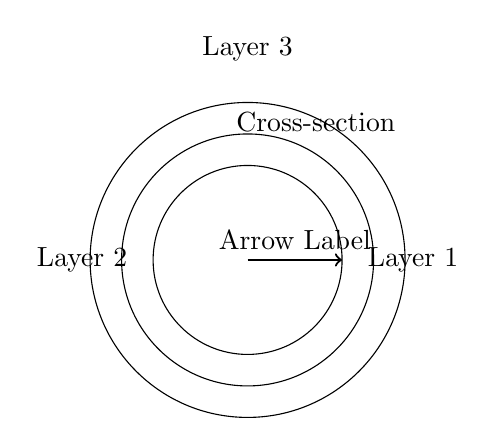
\begin{tikzpicture}[scale=2]
        % Draw the outer circle
        \draw (0, 0) circle (1);

        % Draw the inner circles
        \draw (0, 0) circle (0.8);
        \draw (0, 0) circle (0.6);

        % Add annotations
        \node[anchor=east] at (1.4, 0) {Layer 1};
        \node[anchor=west] at (-1.4, 0) {Layer 2};
        \node[anchor=south] at (0, 1.2) {Layer 3};

        % Add labels
        \node[anchor=north east] at (1, 1) {Cross-section};

        \draw[->, thick] (0, 0) -- (0.6, 0) node[midway, above] {Arrow Label};
    \end{tikzpicture}
    \caption{Cross-section of a sphere with three layers.}
    \label{fig:cross-section}
\end{figure}

\end{document}

